\documentclass[10pt, xcolor=x11names, compress]{beamer}
%\documentclass[10pt, xcolor=x11names, compress, handout]{beamer}
\usetheme{progressbar}
%\usecolortheme[named=Purple4]{structure}
\progressbaroptions{headline=sections,titlepage=normal,frametitle=normal}

\setbeamertemplate{navigation symbols}{}

\usepackage{iwona} 

\usepackage{alltt}
\usepackage{amsmath,amsfonts, amssymb, amscd}
\usepackage{hyperref}
\usepackage{setspace}
\usepackage{wasysym}
\usepackage{ulem}

\usepackage{calc}
\usepackage[overlay,absolute]{textpos}
\TPGrid[5mm,5mm]{20}{20}



\renewcommand{\Re}{\operatorname{Re}}
\renewcommand{\Im}{\operatorname{Im}}
\newcommand{\debye}{\operatorname{debye}}

\newcommand{\chik}{$\chi(k)$}
\newcommand{\chir}{$|\tilde{\chi}(R)|$}


\newcommand{\file}[1]{{\color{Firebrick4}\texttt{`#1'}}}
\newcommand{\multiple}{{\color{Orange3}\textsl{multiple}}}


\newcommand{\atoms}  {{\color{DarkOrchid4}\textsc{atoms}}}
\newcommand{\feff}   {{\color{DarkOrchid4}\textsc{feff}}}
\newcommand{\ifeffit}{{\color{DarkOrchid4}\textsc{ifeffit}}}
\newcommand{\athena} {{\color{DarkOrchid4}\textsc{athena}}}
\newcommand{\artemis}{{\color{DarkOrchid4}\textsc{artemis}}}

\renewenvironment<>{center}
{\begin{actionenv}#1\begin{originalcenter}}
{\end{originalcenter}\end{actionenv}}

\definecolor{guessp}   {rgb}{0.64,0.00,0.64}
\newcommand{\guessp}   {{\color{guessp}guess}}
\definecolor{defp}     {rgb}{0.00,0.55,0.00}
\newcommand{\defp}     {{\color{defp}def}}
\definecolor{setp}     {rgb}{0,0,0}
\newcommand{\setp}     {{\color{setp}set}}
\definecolor{lguessp}  {rgb}{0.24,0.11,0.56}
\newcommand{\lguessp}  {{\color{lguessp}lguess}}
\definecolor{skipp}    {rgb}{0.70,0.70,0.70}
\newcommand{\skipp}    {{\color{skipp}skip}}
\definecolor{restrainp}{rgb}{0.80,0.61,0.11}
\newcommand{\restrainp}{{\color{restrainp}restrain}}
\definecolor{afterp}   {rgb}{0.29,0.44,0.55}
\newcommand{\afterp}   {{\color{afterp}after}}
\definecolor{penaltyp} {rgb}{0.55,0.35,0.17}
\newcommand{\penaltyp} {{\color{penaltyp}penalty}}
\definecolor{mergep}   {rgb}{0.93,0.00,0.00}
\newcommand{\mergep}   {{\color{mergep}merge}}


\mode<presentation>

\title{Modeling non-crystalline samples}

\author{Bruce Ravel}
\institute[NIST]{Synchrotron Methods Group, Materials Measurement Science Division\\%
  Materials Measurement Laboratory\\%
  National Institute of Standards and Technology\\%
  \&\\%
  Local Contact, Beamline X23A2\\%
  National Synchrotron Light Source\\~}


\date[IFPAN, April 2015]{New Challenges and Solutions for XAS Data Analysis\\
  Institute of Physics, Polish Academy of Sciences\\14-17 April, 2015}

\begin{document}
\maketitle

\begin{frame}
  \frametitle{Copyright}
  \tiny

  This document is copyright \copyright 2007-2010 Bruce Ravel.

  \begin{center}
    
\includegraphics[width=1.0cm]{images/somerights20}
  \end{center}

  This work is licensed under the Creative Commons
  Attribution-ShareAlike License.  To view a copy of this license,
  visit \href{http://creativecommons.org/licenses/by-sa/3.0/}
  {\color{Purple4}\texttt{http://creativecommons.org/licenses/by-sa/3.0/}}
  or send a letter to Creative Commons, 559 Nathan Abbott Way,
  Stanford, California 94305, USA.

  \begin{description}
  \item[You are free:] %
    \begin{itemize}
    \item \textbf{to Share} --- to copy, distribute, and transmit the work
    \item \textbf{to Remix} --- to adapt the work
    \end{itemize}
  \item[Under the following conditions:] %
    \begin{itemize}
    \item Attribution. You must attribute the work in the manner
      specified by the author or licensor (but not in any way that
      suggests that they endorse you or your use of the work).
    \item Share Alike. If you alter, transform, or build upon this
      work, you may distribute the resulting work only under the same,
      similar or a compatible license.
    \item Any of these conditions can be waived if you get permission
      from the author.
    \end{itemize}
  \end{description}
  \begin{itemize}
  \item For any reuse or distribution, you must make clear to others
    the license terms of this work. The best way to do this is with a
    link to the URL for this document.
  \item Any of the above conditions can be waived if you get
    permission from the copyright holder.
  \item Nothing in this license impairs or restricts the author's
    moral rights.
  \end{itemize}

  Your fair dealing and other rights are in no way affected by the
  above.  This is a human-readable summary of the Legal Code (the full
  license).


\end{frame}

%%% Local Variables:
%%% mode: latex
%%% TeX-master: "pimst2"
%%% End:



\section[Introduction]{Introduction}
\begin{frame}
  \frametitle{Introduction}
  Earlier I demonstrated {\artemis} by showing FeS$_2$, which is a
  crystal.  This allowed me to start with {\atoms} and crystal data.

  \begin{alertblock}{Atoms is just a tool}
    It is useful when it's useful.
  \end{alertblock}

  In this short talk, I will suggest various ways to get started on
  samples that are not crystalline.
\end{frame}

\section{Germanium}
\label{sec:ge}

\begin{frame}[fragile]
  \frametitle{Crytsalline and amorphous germanium}
  \begin{columns}
    \begin{column}{0.30\linewidth}
      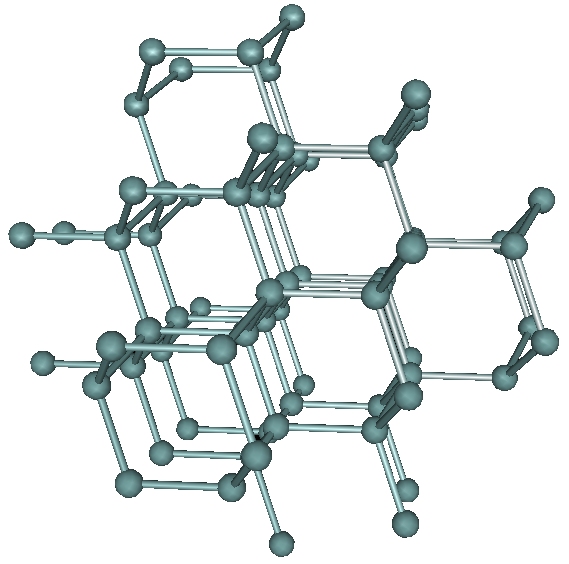
\includegraphics[width=\linewidth]{images/cGe.png}\\
      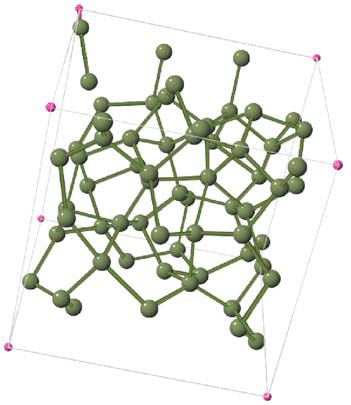
\includegraphics[width=\linewidth]{images/aGe.png}
    \end{column}
    \begin{column}{0.7\linewidth}
      Ge crystalizes into an orderly, hexagonal close pack
      arrangement.  Given EXAFS data on the crystalline material, it
      is fairly obvious how to begin: Run {\feff} starting from the
      known crystal data.
      \begin{center}
        \begin{minipage}{0.5\linewidth}
\begin{alltt}
\scriptsize
{\color{SteelBlue2}space} = f d 3 m
{\color{Purple2}a}     = 5.658
{\color{Purple2}rmax}  = 6.00
{\color{Brown4}atoms}
  Ge   1/8   1/8   1/8
\end{alltt}
        \end{minipage}
      \end{center}
      Amorphous Ge is a random continuous network.  

      \medskip

      \begin{alertblock}<2-3>{}
        Do we have to run a molecular dynamics simulation just to
        then run {\feff}?

        \smallskip

        \onslide<3>{\raggedleft Happily, no.}
      \end{alertblock}
    \end{column}
  \end{columns}

  \begin{bottomnote}[0.5][19.25]
    aGe figure from
    V.\ Hugouvieux et al PRB \textbf{75}, 104208 (2007)
    \doiref{10.1103/PhysRevB.75.104208}[LightBlue4]
  \end{bottomnote}
  
\end{frame}
\begin{frame}
  \frametitle{Crytsalline and amorphous germanium}

  As always, let's start by looking at the data.

  \bigskip

  \begin{columns}
    \begin{column}{0.33\linewidth}
      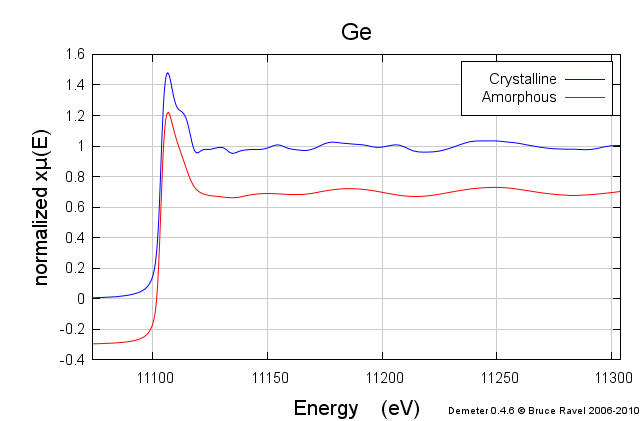
\includegraphics[width=\linewidth]{images/Ge_mu.png}
    \end{column}
    \begin{column}{0.33\linewidth}
      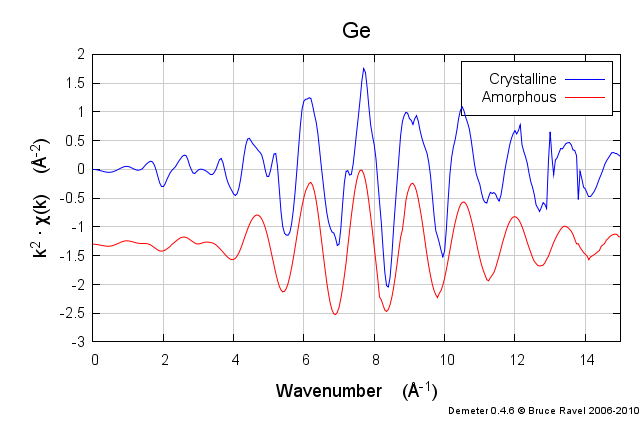
\includegraphics[width=\linewidth]{images/Ge_chik.png}
    \end{column}
    \begin{column}{0.33\linewidth}
      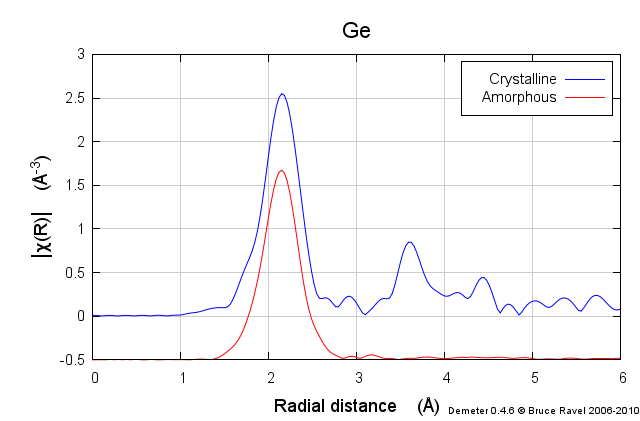
\includegraphics[width=\linewidth]{images/Ge_chir.png}
    \end{column}
  \end{columns}

  \bigskip

  A random continuous network has a near-neighbor pair correlation
  nearly identical to its ordered counterpart.  We see this behavior
  in our Ge data.
  \begin{bottomnote}[0.5][19.25]
    Amorphous data is courtesy of Joe Woicik and was measured at NSLS
    X23A2.  Crystalline data taken from the NSLS X18A website.
  \end{bottomnote}
  
\end{frame}

\begin{frame}[fragile]
  \frametitle{Fit to aGe}
  \begin{columns}
    \begin{column}{0.4\linewidth}
      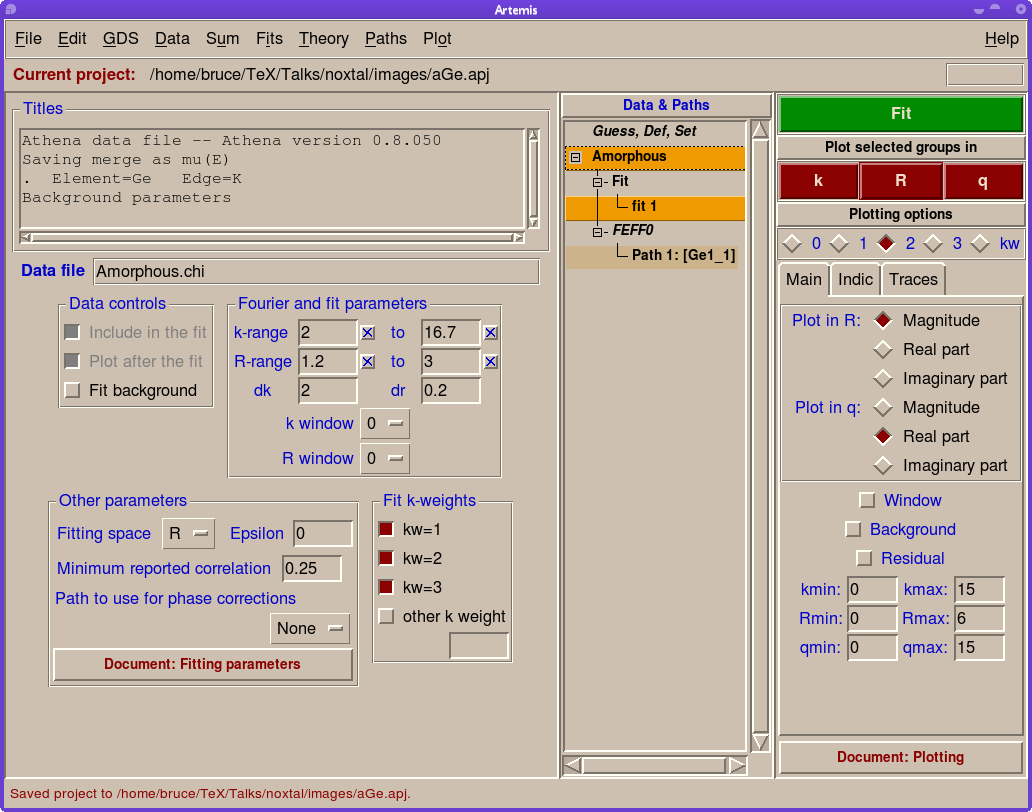
\includegraphics[width=\linewidth]{images/aGe_fit.png}\\[2ex]
      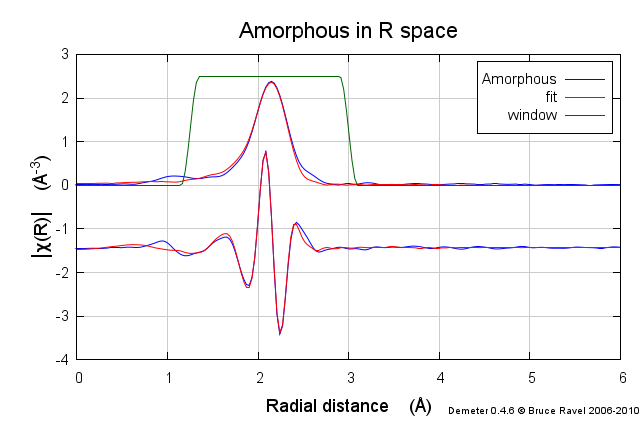
\includegraphics[width=\linewidth]{images/aGe_fit_chir.png}
    \end{column}
    \begin{column}{0.6\linewidth}
      We import the data and the first path from the {\feff}
      calculation on crystalline Ge.

      \medskip

      We make a simple, first shell fitting model with terms for
      $S_0^2$, $\Delta E_0$, $\Delta R$, and $\sigma^2$.
      \begin{center}
        \begin{minipage}{0.8\linewidth}
          \begin{exampleblock}{}
\begin{alltt}
\scriptsize
guess parameters:                                                            
  amp   =   1.10      +/-   0.07
  enot  =   3.94      +/-   0.75
  delr  =   0.006     +/-   0.004
  ss    =   0.00596   +/-   0.00040
\end{alltt}
          \end{exampleblock}

        \end{minipage}
      \end{center}
      We find that the bond length and coordination number for aGe is
      much the same as for cGe, while the disorder is a bit higher.
    \end{column}
  \end{columns}
\end{frame}
\section{Molecule}
\label{sec:molecule}

\begin{frame}
  \frametitle{Molecule file formats}
  Just because a material is not a crystal does not mean that its
  structure is not known.  Atomic structures of molecules from
  coordination complexes up to biological macromolecules are known
  from theory and experiment and are available in a variety of file
  formats.

  \bigskip

  \begin{block}{}
    \begin{center}
      {\feff} needs a list of cartesian coordinates.
    \end{center}
  \end{block}

  \bigskip

  Sadly, the current version of {\artemis} cannot help you convert a
  molecule file into a \file{feff.inp} file, but it is not hard.
\end{frame}

\begin{frame}
  \frametitle{Methyl tin chloride}
  One of my standard teaching examples involves Sn K edge data on
  methyl tin chloride dissolved in an organic solvent.

  \begin{columns}
    \begin{column}{0.5\linewidth}
      \begin{center}
        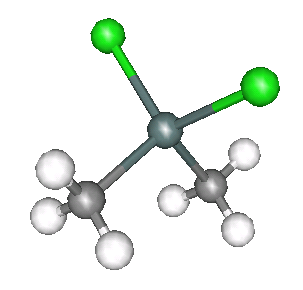
\includegraphics[width=0.5\linewidth]{images/dimethyltin_dichloride.png}\\
      Dimethyl tin dichloride
      \end{center}
    \end{column}
    \begin{column}{0.5\linewidth}
      \begin{center}
        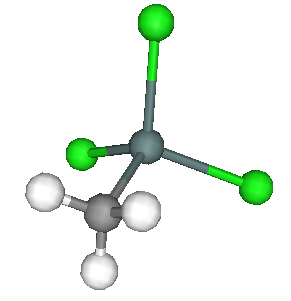
\includegraphics[width=0.5\linewidth]{images/monomethyltin_trichloride.png}\\
        Monomethyl tin trichloride
      \end{center}
    \end{column}
  \end{columns}
  \begin{columns}
    \begin{column}{0.33\linewidth}
      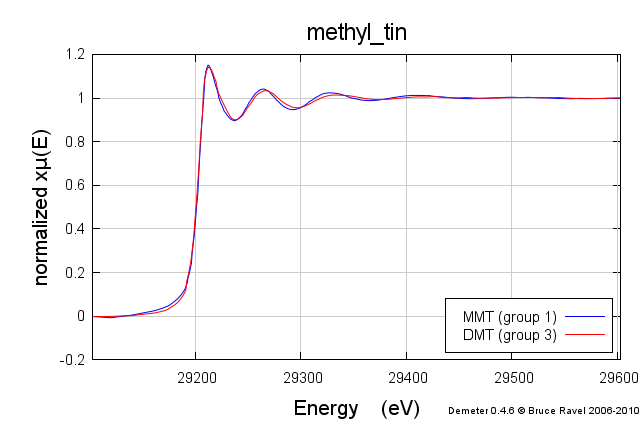
\includegraphics[width=\linewidth]{images/mtin_mu.png}
    \end{column}
    \begin{column}{0.33\linewidth}
      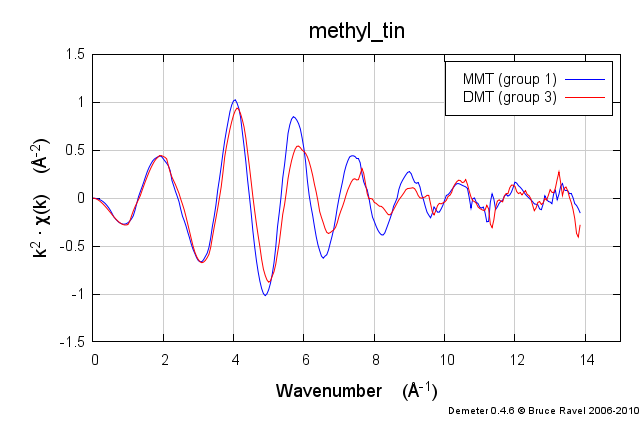
\includegraphics[width=\linewidth]{images/mtin_chik.png}
    \end{column}
    \begin{column}{0.33\linewidth}
      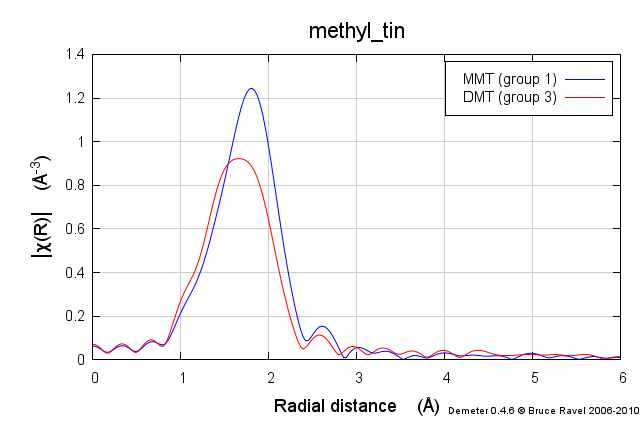
\includegraphics[width=\linewidth]{images/mtin_chir.png}
    \end{column}
  \end{columns}
\end{frame}


\begin{frame}[fragile]
  \frametitle{Protein Data Bank file format}
  A bit of googling turned up a structure for dimethyl tin dichloride
  in the form of a PDB file.  It looks like this:

  \begin{block}{}
\begin{alltt}
\scriptsize
COMPND    5261536
HETATM    1 \alert{ C}1  LIG     1      \alert{-0.027   2.146   0.014}  1.00  0.00
HETATM    2 \alert{SN}2  LIG     1      \alert{ 0.002  -0.004   0.002}  1.00  0.00
HETATM    3 \alert{ C}3  LIG     1      \alert{ 1.042  -0.716   1.744}  1.00  0.00
HETATM    4 \alert{CL}4  LIG     1      \alert{-2.212  -0.821   0.019}  1.00  0.00
HETATM    5 \alert{CL}5  LIG     1      \alert{ 1.107  -0.765  -1.940}  1.00  0.00
HETATM    6 1\alert{H}1  LIG     1      \alert{ 0.996   2.523   0.006}  1.00  0.00
HETATM    7 2\alert{H}1  LIG     1      \alert{-0.554   2.507  -0.869}  1.00  0.00
HETATM    8 3\alert{H}1  LIG     1      \alert{-0.537   2.497   0.911}  1.00  0.00
HETATM    9 1\alert{H}3  LIG     1      \alert{ 0.532  -0.365   2.641}  1.00  0.00
HETATM   10 2\alert{H}3  LIG     1      \alert{ 1.057  -1.806   1.738}  1.00  0.00
HETATM   11 3\alert{H}3  LIG     1      \alert{ 2.065  -0.339   1.736}  1.00  0.00
END
\end{alltt}
  \end{block}

The \alert{red bits} are atomic species and cartesian coordinates ---
just what we need!
\end{frame}

\begin{frame}[fragile]
  \frametitle{Feff6 input file}
  \begin{columns}
    \begin{column}{0.45\linewidth}
\begin{alltt}
\scriptsize
 {\color{Green4}TITLE dimethyltin dichloride}
 {\color{Purple2}HOLE}      1   1.0  {\color{Blue4} *  Sn K edge (29200 eV), S0^2}
 {\color{Blue4}*         mphase,mpath,mfeff,mchi}
 {\color{SteelBlue2}CONTROL}   1      1     1     1
 {\color{SteelBlue2}PRINT}     1      0     0     0
 {\color{Purple2}RMAX}      6.0

 {\color{Brown4}POTENTIALS}
 {\color{Blue4}*    ipot   Z  element}
        0   50   Sn        
        1   17   Cl
        2    6   C
        3    1   H
 {\color{Brown4}ATOMS}
 {\color{Blue4}*   x       y       z    ipot}
   -0.027   2.146   0.014  2
    0.002  -0.004   0.002  0
    1.042  -0.716   1.744  2
   -2.212  -0.821   0.019  1
    1.107  -0.765  -1.940  1
    0.996   2.523   0.006  3
   -0.554   2.507  -0.869  3
   -0.537   2.497   0.911  3
    0.532  -0.365   2.641  3
    1.057  -1.806   1.738  3
    2.065  -0.339   1.736  3
\end{alltt}      
    \end{column}
    \begin{column}{0.55\linewidth}
      ~\\[2ex]

      \begin{enumerate}
      \item Prepare \file{feff.inp} boilerplate
      \item Cut-n-paste the cartesian coordinates in the
        {\color{Brown4}\texttt{ATOMS}} list
      \item Make a {\color{Brown4}\texttt{POTENTIALS}} list out the
        atomic species
      \item The absorber \textbf{must} be potential \#0, but it need
        be neither first in the {\color{Brown4}\texttt{ATOMS}} list
        nor be at (0,0,0)
      \item The {\color{Brown4}\texttt{ATOMS}} list need not be in
        order of radial distance (or any other order)
      \item This \file{feff.inp} file can be imported directly into
        {\artemis}
      \end{enumerate}
    \end{column}
  \end{columns}
\end{frame}


\begin{frame}
  \frametitle{Now do a fit}

  Import each data set and one {\feff} calculation into \artemis.  Use
  the relevant paths with each data set.
  \begin{columns}
    \begin{column}{0.5\linewidth}
      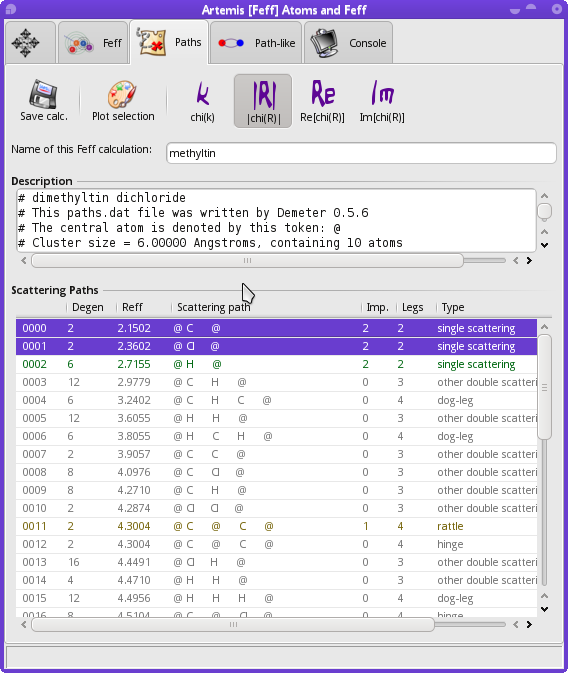
\includegraphics[width=0.85\linewidth]{images/mtin_intrp.png}
      %
      %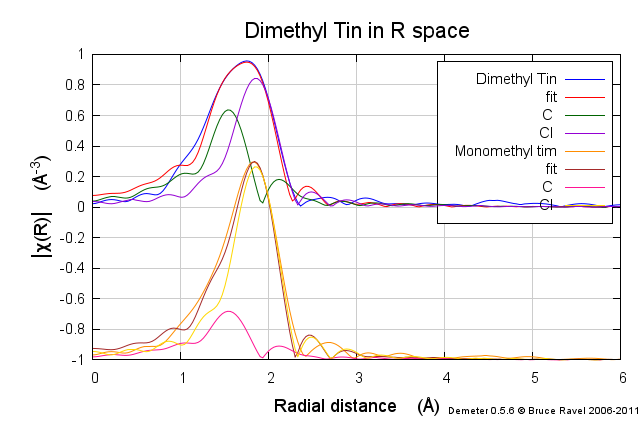
\includegraphics[width=0.7\linewidth]{images/mtin_fit_chir.png}
    \end{column}
    \begin{column}{0.5\linewidth}
      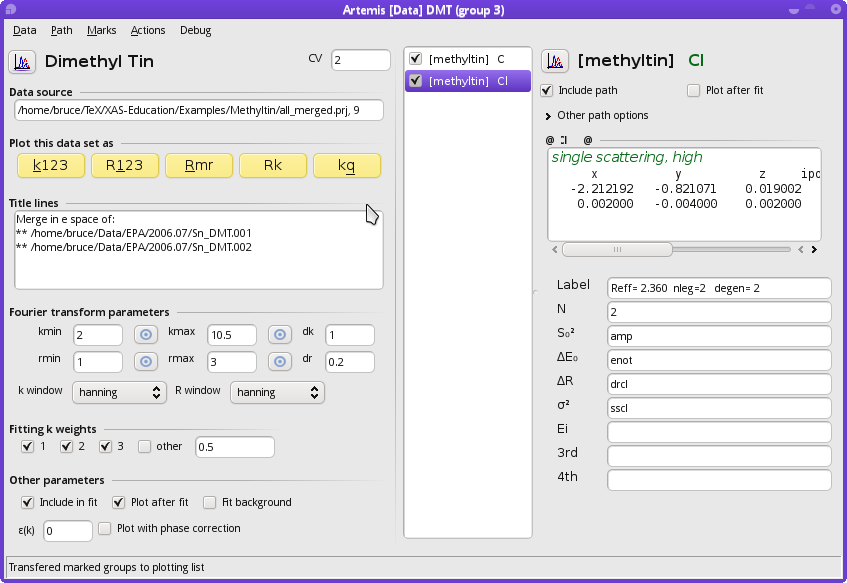
\includegraphics[width=0.8\linewidth]{images/mtin_fit.png}

      \smallskip

      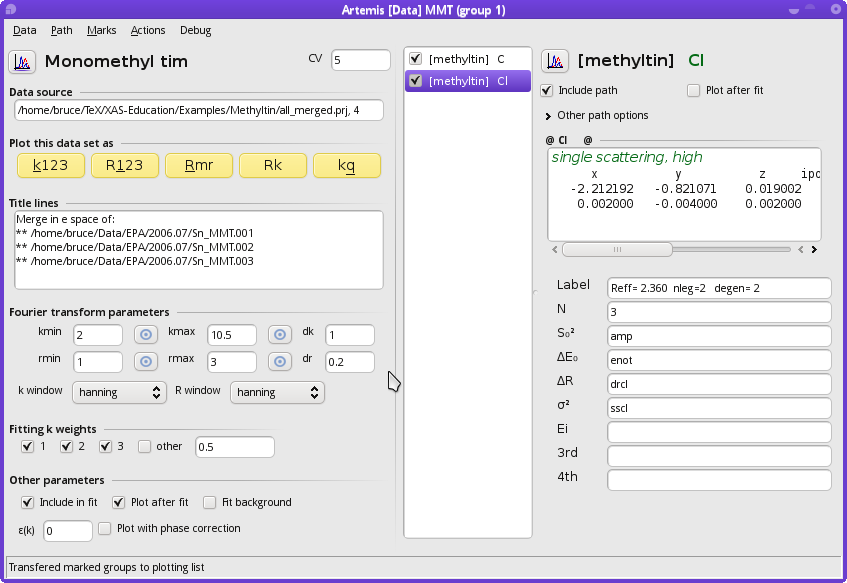
\includegraphics[width=0.8\linewidth]{images/mtin_fit2.png}
    \end{column}
  \end{columns}
  \begin{bottomnote}[0.5][19.25]
    This is the topic of the next demo.
  \end{bottomnote}
\end{frame}

\begin{frame}
  \frametitle{How could this be made better?}
  \begin{columns}
    \begin{column}{0.2\linewidth}
      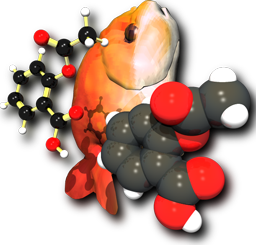
\includegraphics[width=\linewidth]{images/babel256.png}
    \end{column}
    \begin{column}{0.8\linewidth}
      Open Babel (\href{http://openbabel.org/}
      {\color{Blue2}\texttt{http://openbabel.org/}}) is a chemical
      toolbox that, among other things, translates between 98
      different atomic structure file formats.
    \end{column}
  \end{columns}
  \begin{block}{Integrating Open Babel with {\feff} and {\artemis}}
    \begin{enumerate}
    \item Open Babel is written in C++
    \item File format I/O is handled by small extension modules, also
      written in C++
    \item Need a \file{feff.inp} I/O module written and donated to the
      Open Babel project
    \item Integrate Open Babel into {\artemis}
    \end{enumerate}
  \end{block}
  \begin{alertblock}<2>{This has long been on my to do list.}
    This is a substantive, yet tractable, way that someone could make
    a contribution to the {\ifeffit} project.

    \smallskip

    \textit{Any volunteers?}
  \end{alertblock}
\end{frame}

\section{Sorbed Uranyl Acetate}
\label{sec:uace}

\begin{frame}
  \frametitle{Sorbed species}
  \begin{block}{Here's a paper you should read}
    \small
    \textit{X-ray absorption fine structure determination of
      pH-dependent U-bacterial cell wall interactions}, %
    S.D.\ Kelly, et al. Geochimica et Cosmochimica Acta \textbf{66}:22
    (2002) 3855-3871
    \doiref{10.1016/S0016-7037(02)00947-X}
  \end{block}

  \medskip

  In it, the authors measure the pH dependence of the cell wall
  functional groups responsible for the absorption of aqueous
  UO$_2^{2+}$ to \textit{B. subtilis} from pH 1.67 to 4.80.

  \begin{center}
    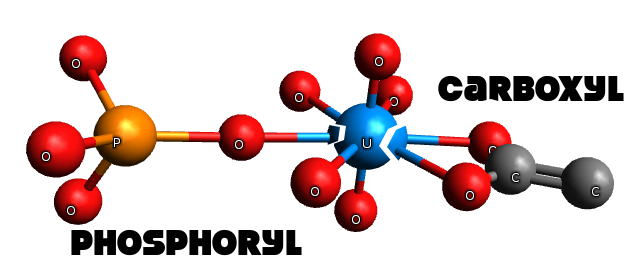
\includegraphics[width=0.6\linewidth]{images/uranyl.png}
  \end{center}
\end{frame}


\begin{frame}
  \frametitle{Using crystal analogs as Feff structures}
  \small
  \begin{columns}[T]
    \begin{column}{0.5\linewidth}
      Triuranyl diphoshate tetrahydrate contains a monodentate U-P moiety.
    \end{column}
    \begin{column}{0.5\linewidth}
      Sodium uranyl triacetate contains a bidentate U-C moiety.
    \end{column}
  \end{columns}

  \smallskip

  \begin{columns}[T]
    \begin{column}{0.5\linewidth}
      \begin{center}
        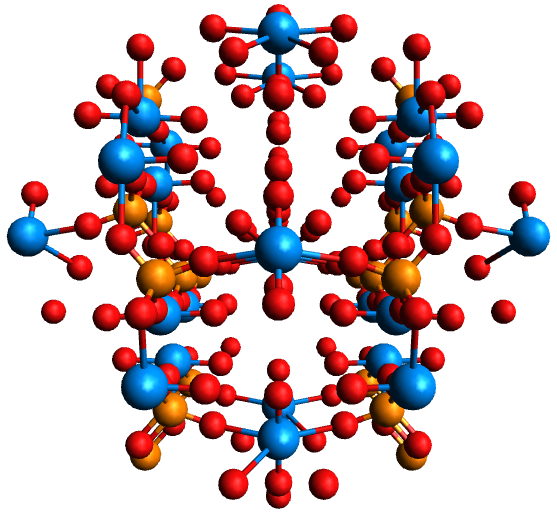
\includegraphics[width=0.6\linewidth]{images/upo4.png}

        \onslide<2>{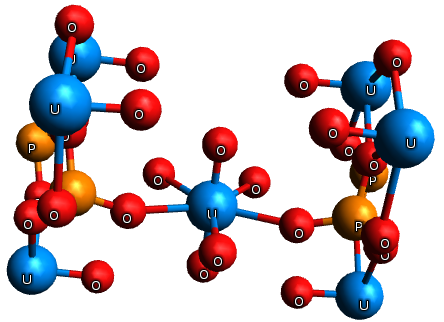
\includegraphics[width=0.7\linewidth]{images/upo4_full.png}}
      \end{center}
    \end{column}
    \begin{column}{0.5\linewidth}
      \begin{center}
        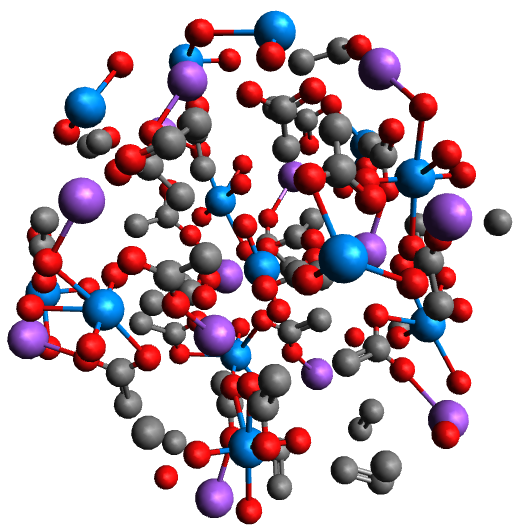
\includegraphics[width=0.6\linewidth]{images/NaU_triacetate_full.png}

        \onslide<2>{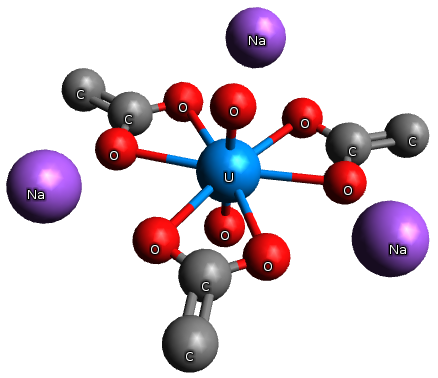
\includegraphics[width=0.65\linewidth]{images/NaU_triacetate.png}}
      \end{center}
    \end{column}
  \end{columns}
\end{frame}

\begin{frame}
  \frametitle{Choosing paths selectively from crystal analogs}
  \small
  \begin{columns}[T]
    \begin{column}{0.5\linewidth}
      \begin{center}
        The monodentate U-P from the crystal resembles the phoshporyl
        coordination structure we are looking for:

        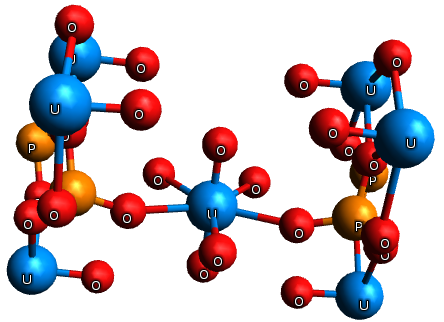
\includegraphics[width=0.7\linewidth]{images/upo4_full.png}
      \end{center}
    \end{column}
    \begin{column}{0.5\linewidth}
      \begin{center}
        The bidentate U-C from the crystal resembles the carboxyl
        coordination structure we are looking for:

        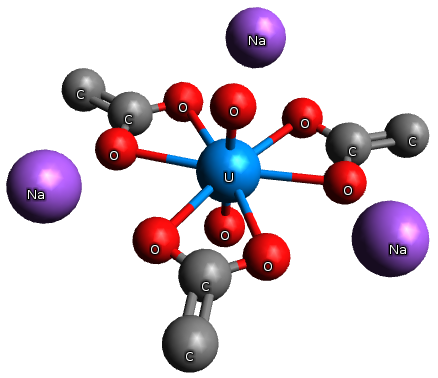
\includegraphics[width=0.65\linewidth]{images/NaU_triacetate.png}
      \end{center}
    \end{column}
  \end{columns}
  \begin{center}
    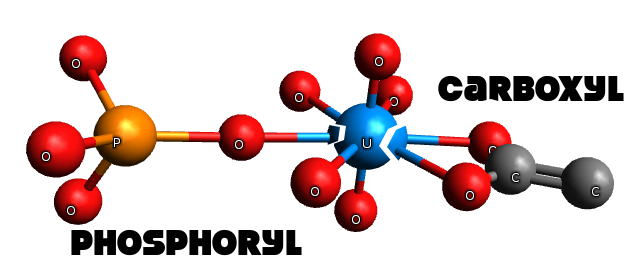
\includegraphics[width=0.6\linewidth]{images/uranyl.png}
  \end{center}
\end{frame}

\begin{frame}
  \frametitle{The moral of this story}
  \begin{block}{The practical version}
    The structure used in the {\feff} calculation doesn't need to be
    ``perfect''.  Close is usually good enough to get started.
  \end{block}

  \medskip

  \begin{alertblock}<2>{The technical version}
    Small changes in local coordination do not result in large changes
    to the complex scattering factor ($F(k)$ and $\Phi(k)$ in the
    EXAFS equation).  EXAFS \alert{\textbf{is}} sensitive to small
    changes in local coordination, but this is due to the $\sin(2kR)$
    term.

    \smallskip

    A high quality EXAFS analysis can suffer an approximation to the
    local coordination environment in the calculation of the
    thoeretical fitting standards so long as the fitting model is
    parameterized in a way to capture the details of that local
    coordination.
  \end{alertblock}
\end{frame}

\begin{frame}
  \frametitle{Using crystal analogs in Artemis}
  \begin{columns}[b]
    \begin{column}{0.33\linewidth}
      \begin{center}
        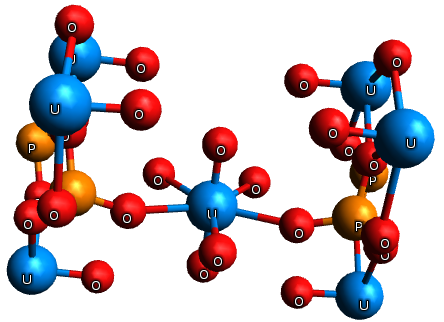
\includegraphics[width=0.7\linewidth]{images/upo4_full.png}
      \end{center}
    \end{column}
    \begin{column}{0.33\linewidth}
      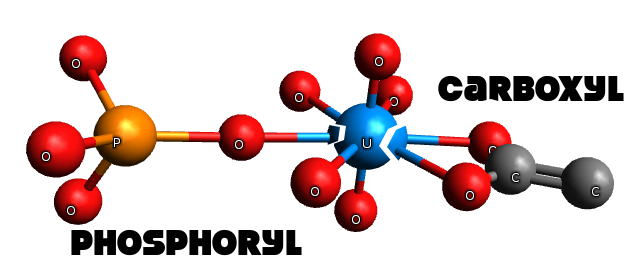
\includegraphics[width=\linewidth]{images/uranyl.png}
    \end{column}
    \begin{column}{0.33\linewidth}
      \begin{center}
        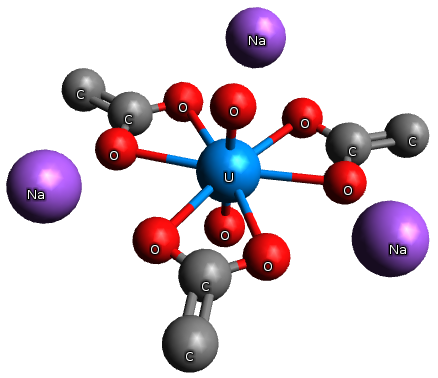
\includegraphics[width=0.65\linewidth]{images/NaU_triacetate.png}
      \end{center}
    \end{column}
  \end{columns}

  \bigskip

  Here's the outline:
  \begin{enumerate}
  \item Import each crystal structure into {\artemis}
  \item Run {\atoms}, run {\feff}
  %\item Choose the ``Import no paths'' option when asked
  \item Examine the path list, select those SS and MS paths you need
    to describe your structure
  \item Parameterize, fit
  \end{enumerate}
\end{frame}


\section{Take-home messages}
\label{sec:takehome}

\begin{frame}
  \frametitle{Take-home messages}
  \begin{description}[<+->][Close is]
  \item[Close is probably good enough] ~\\Running {\feff} on a structure
    that resembles the actual data is usually adequate.  More
    technically --- the computation of the scattering factor is not
    acutely sensitive to atomic positions.
  \item[Be creative] ~\\What makes an \textit{expert} practitioner is
    the ability to conceive of and implement an analytical strategy.
    There is no rule book (sadly) -- new problems bring new
    challenges.  An expert is just someone who sees an interesting
    idea through to completion.
  \item[You never know nothing] ~\\Use your prior knowledge of your
    sample.  If you have a hunch (even a weak suspicion) about the
    local configuration, you have enough to get started with {\feff}.
  \item[Some information is better than no information] ~\\At the end
    of the day, you may only be able to extract a little bit of
    information about the local configuration.  Scientific progress is
    made in tiny steps.
  \end{description}
\end{frame}


\end{document}

%%% Local Variables:
%%% mode: latex
%%% TeX-master: t
%%% TeX-parse-self: t
%%% TeX-auto-save: t
%%% TeX-auto-untabify: t
%%% TeX-PDF-mode: t
%%% End:
